%# -*- coding: utf-8-unix -*-
% !TEX program = xelatex
% !TEX root = ../thesis.tex
% !TEX encoding = UTF-8 Unicode
%%==================================================
%% chapter02.tex for SJTU Master Thesis
%% based on CASthesis
%% modified by wei.jianwen@gmail.com
%% Encoding: UTF-8
%%==================================================


\chapter{Competition on two layer with various structural network}
\label{chap:competition on two layer with various structural network}
In this chapter, based on the competition model described in chapter. ~\ref{chap:modeling and analysis methods}, simulation would be implemented with changing the network structures. As the basic model, interconnected layers with random regular network would be provided. And then, the interconnected network structure would be altered by changing the internal edges, external edges and network types. Finally, all simulations would be compared and analyzed with the indexes, \textit{AS total}, \textit{PCR}, \textit{NCR} and \textit{CR}

\section{Competition on Random Regular Networks}
\label{competition on Random Regular Networks}
\begin{figure}[!h]
	\centering
	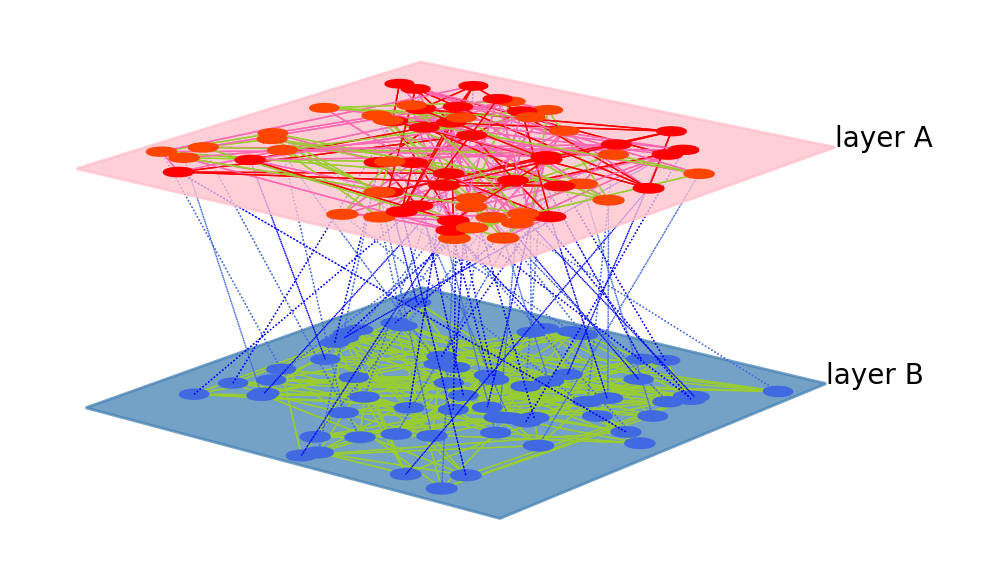
\includegraphics[width=\hsize]{chap3_RR(5)_RR(5).png}
	\caption{Competition on random regular network}
	\label{chap3_RR(5)_RR(5)}
\end{figure}
\begin{figure}[!h]
	\centering
	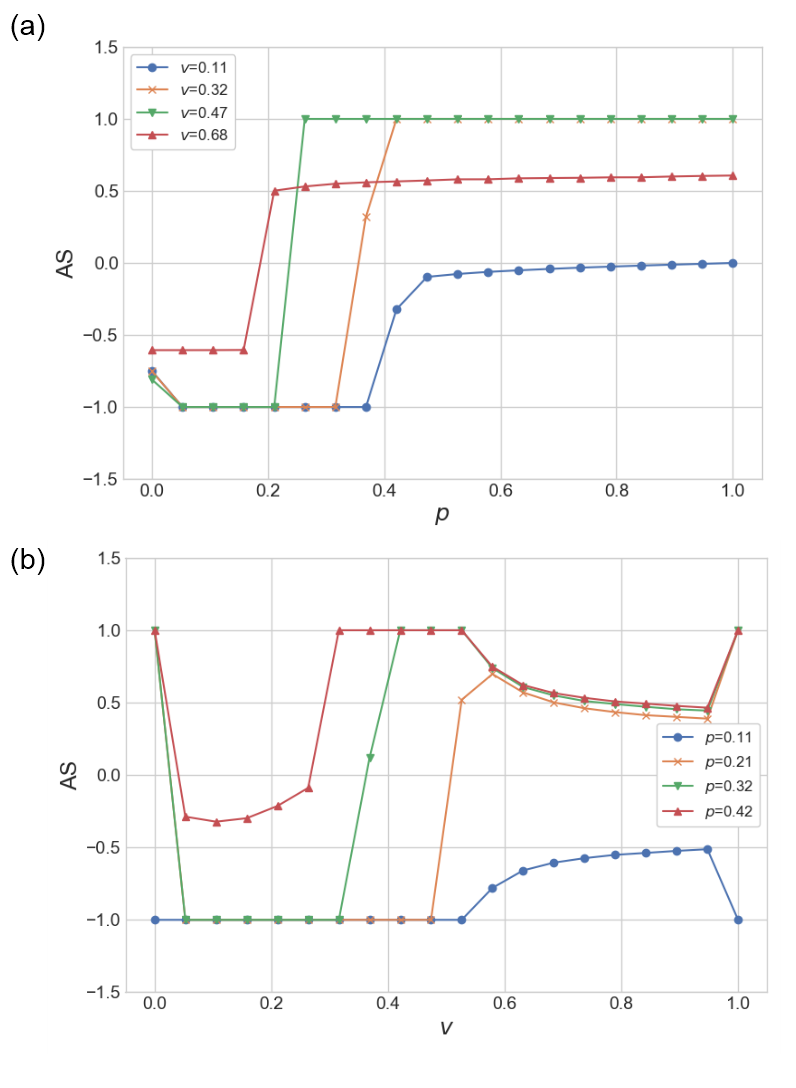
\includegraphics[width=\hsize]{chap3_RR(5)_RR(5)_2d.png}
	\caption{(a) $p$-\textit{AS} chart according to certain $v$ values. (b) $v$-\textit{AS} chart according to certain $p$ values.}
	\label{chap3_RR(5)_RR(5)_2d}
\end{figure}
\begin{figure}[!h]
	\centering
	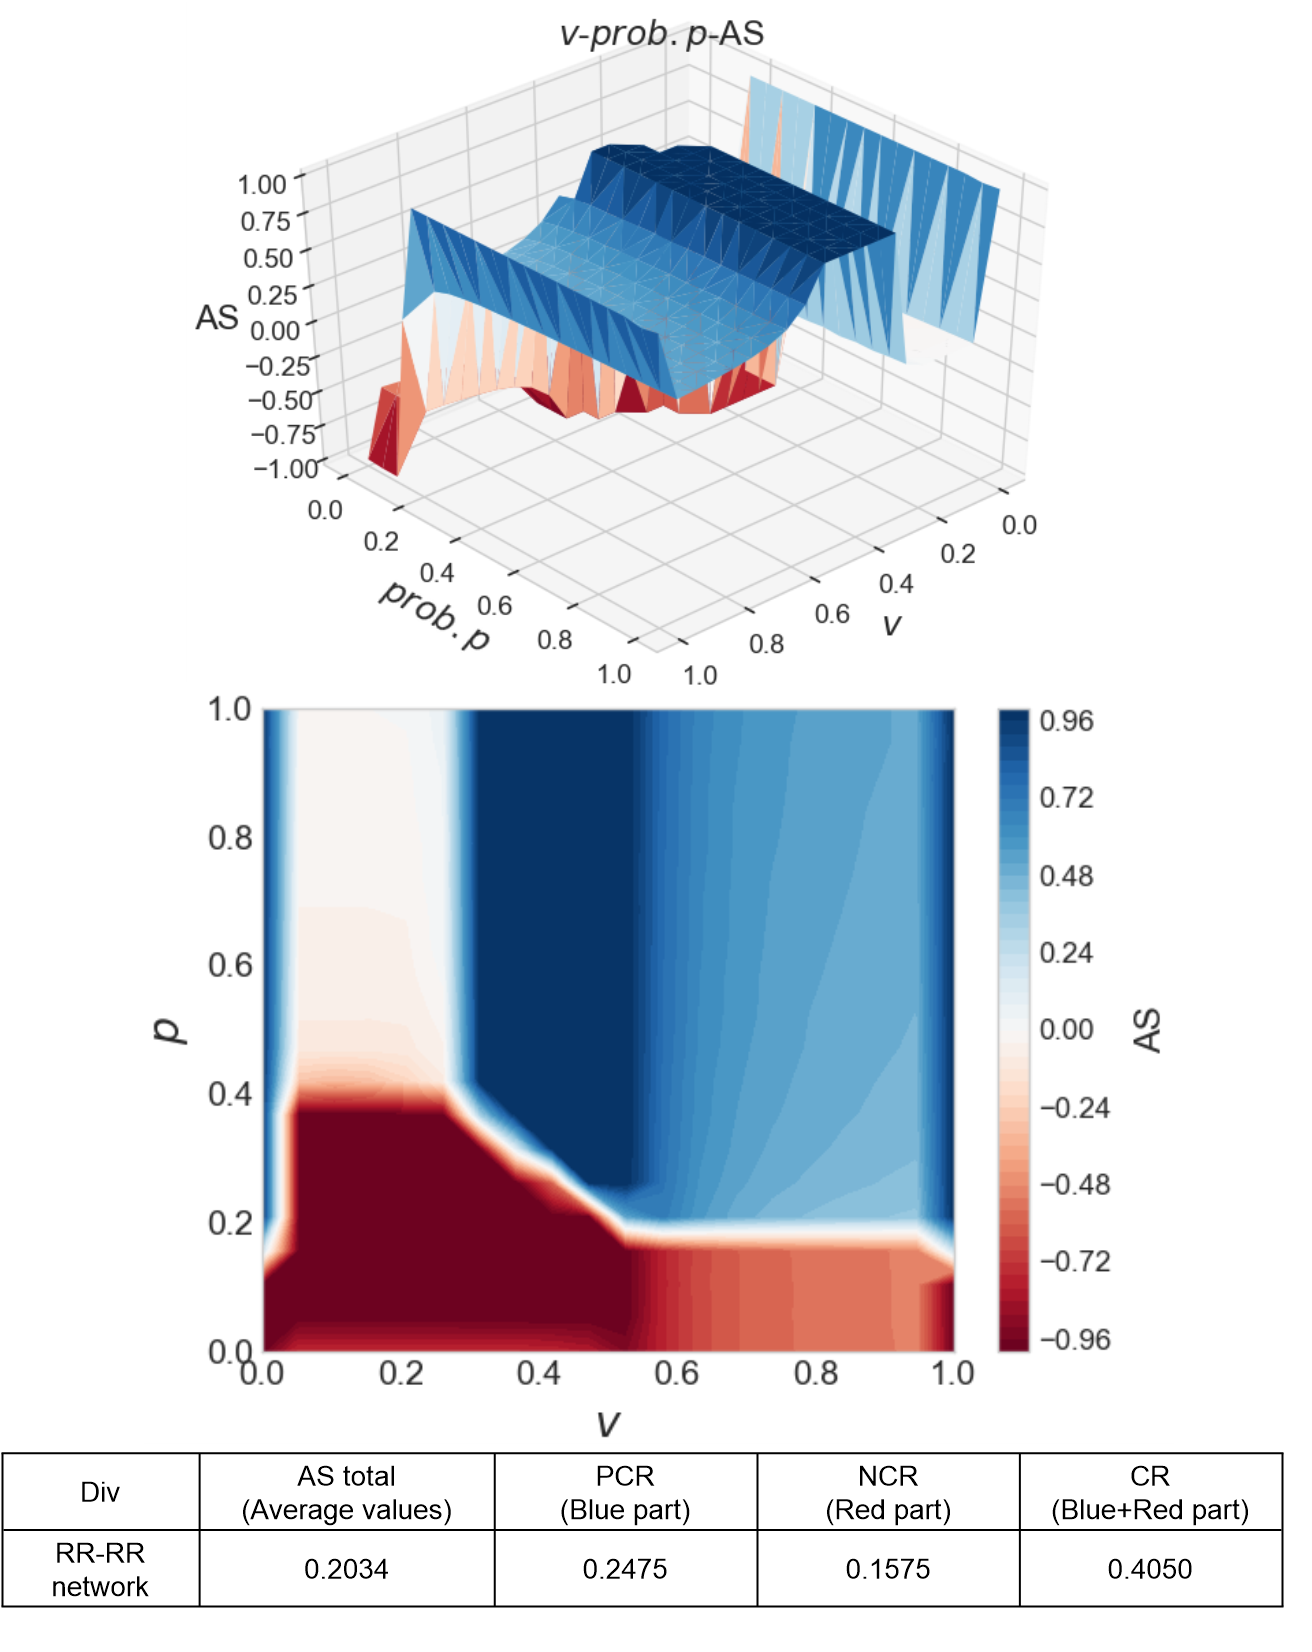
\includegraphics[width=\hsize]{chap3_RR(5)_RR(5)_total.png}
	\caption{\textit{AS} with changing with all $p$ and $v$}
	\label{chap3_RR(5)_RR(5)_total}
\end{figure}
In this section, simulation results on random regular network would be provided to comprehend the competition of two layers. Each layer consists of random regular network that has $N$ nodes with $k$ internal edges as introduced in \parencite{kimsangwoo2012, choi2011, bela2001}. Each node of one layer is connected with a random node on the other layer. This means each node has only $1$ external un-directed edge. Simulations are preformed on network with $N=2048$, and $k = 5$. 

The simulation results are shown in Fig.~\ref{chap3_RR(5)_RR(5)_2d} and Fig.~\ref{chap3_RR(5)_RR(5)_total}.  Fig.~\ref{chap3_RR(5)_RR(5)_2d} presents that how the Average State(\textit{AS}) are changed according to each parameter, $p$ and $v$. So we can know that how each parameter works on the network. Fig.~\ref{chap3_RR(5)_RR(5)_total} provides total results with all parameters. Through these figures, the characteristics of network would be analyzed.

Fig.~\ref{chap3_RR(5)_RR(5)_2d}(a) shows that when $p > 0.2$, $0.32 < v < 0.47$, it normally tends to positive consensus. But, if $v$ is lower or larger than certain values, it doesn't make consensus.
In Fig.~\ref{chap3_RR(5)_RR(5)_2d}(b), as $v$ increases, it normally change from negative to positive consensus. But, when $p$ is very low($p \le 0.11$), it doesn't make positive consensus. On the other hand, when $p$ is large enough, it makes positive consensus. But, when $v$ is small enough, it is changed into negative consensus. When both of $p$ and $v$ are large enough, the state is in a coexistence part.

Fig.~\ref{chap3_RR(5)_RR(5)_total} shows the states of two layers according to all $p$s and all $v$s. As previously described in chapter.~\ref{chap:modeling and analysis methods}, blue area is for positive consensus, red area is for negative consensus, and light colored and white area is for coexistence. And indexes for consensus are also measured.Positive consensus area is 0.2475, and negative consensus area is 0.1575. Coexistence area is $1 - CR = 0.5950$. By using these values and figures, this model would be compared with various structural networks in next section. Through these charts, several facts can be arranged. First, large $p$ tends to make positive consensus and small $p$ tends to make negative consensus. Second, small $v$ tends to make negative consensus, and large $v$ tends to make coexistence state. 

\section{Competition on Networks with different number of external links}
\begin{figure}[!htb]
	\centering
	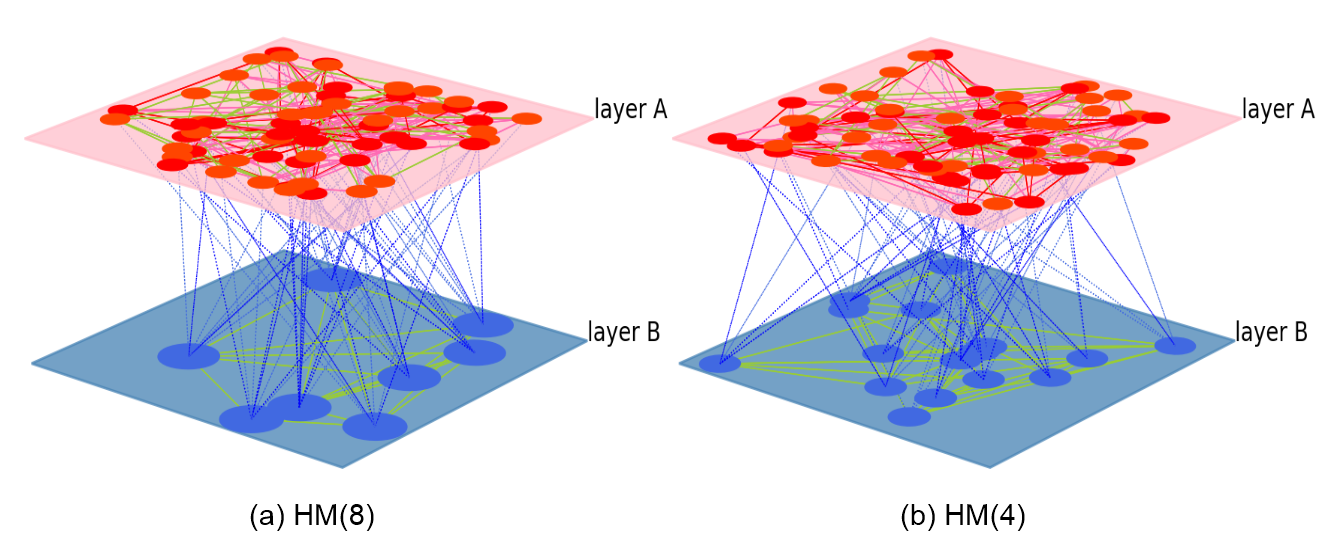
\includegraphics[width=\hsize]{chap3_HM.png}
	\caption{Competition on hierarchical model}
	\label{chap3_HM}
\end{figure}
In this section, we consider the influence of external links. Based on the basic model in section~\ref{competition on Random Regular Networks}, we reduce the number of nodes in layer B at a certain rate and increase the external links from nodes in layer B accordingly as shown in Fig.~\ref{chap3_HM}.  We denote \textit{HM(n)} as a hierarchical model with a level $n$, which means that the number of nodes in layer B is $1/n$ of the number of nodes in layer A, and the number of external links from node in layer B is $n$ in view that the number of external links from node in layer A is $1$. In other words, each node in layer A has one external edge, but each node in layer B has $n$ external edges for \textit{HM(n)}, which means one node in layer B can be influenced by $n$ nodes in layer A.
\begin{figure}[!htb]
	\centering
	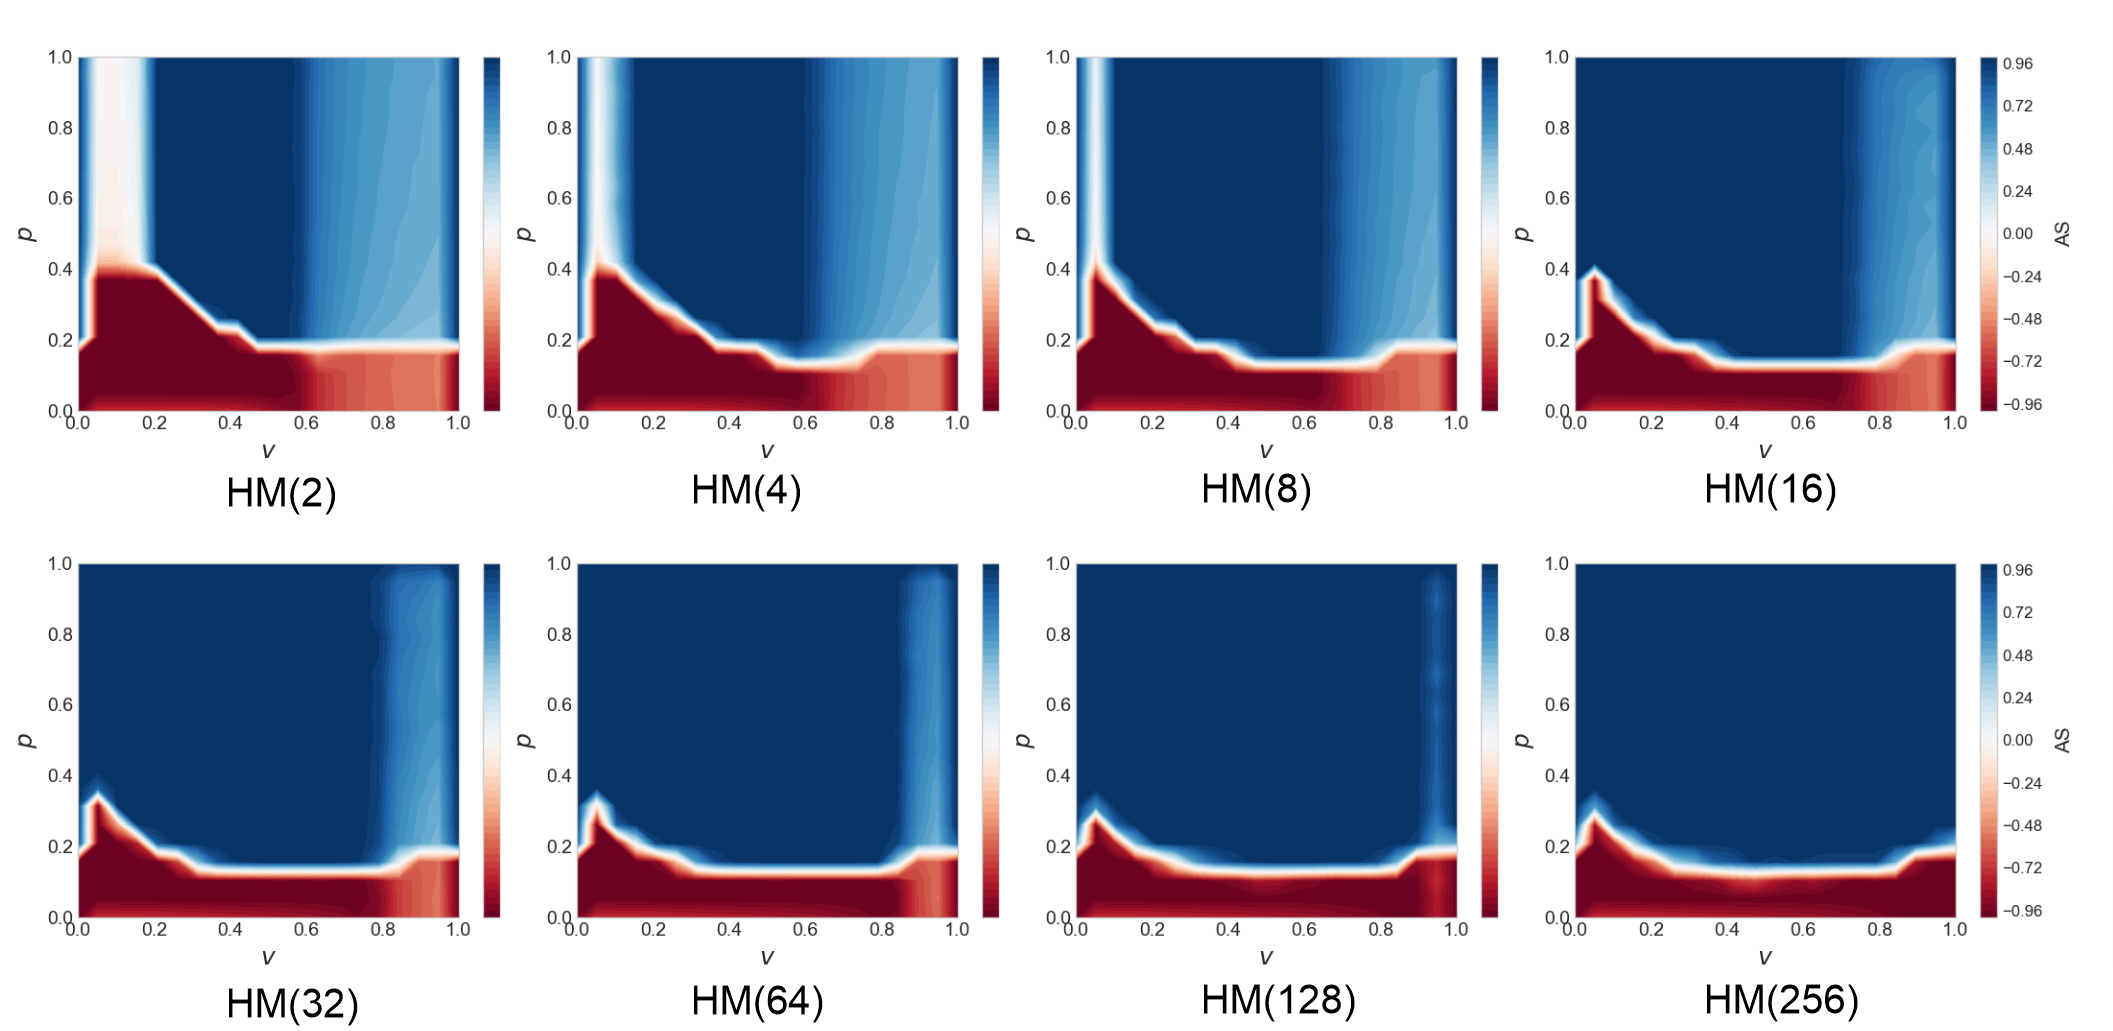
\includegraphics[width=\hsize]{chap3_HMs_AStotal.png}
	\caption{\textit{AS total} on various hierarchical models}
	\label{chap3_HMs_AStotal}
\end{figure}
To find out the significant influence of external edges, various \textit{HM(n)s} were simulated.  Totally, $8$ \textit{HM(n)}, \textit{HM(2), HM(4), HM(8), HM(16), HM(32), HM(64), HM(128), HM(256)} were arranged as shown in Fig.~\ref{chap3_HMs_AStotal}.  
Fig.~\ref{chap3_HMs_AStotal} shows that \textit{HM(2)} has the most area for coexistence part(light and white area) and \textit{HM(256)} has the most are for consensus part(blue and red area). As $n$ in \textit{HM(n)} is increased, coexistence area is decreased and consensus area is increased. Particularly, positive consensus area is significantly increased, negative consensus area is slightly decreased.  
\begin{figure}[!htb]
	\centering
	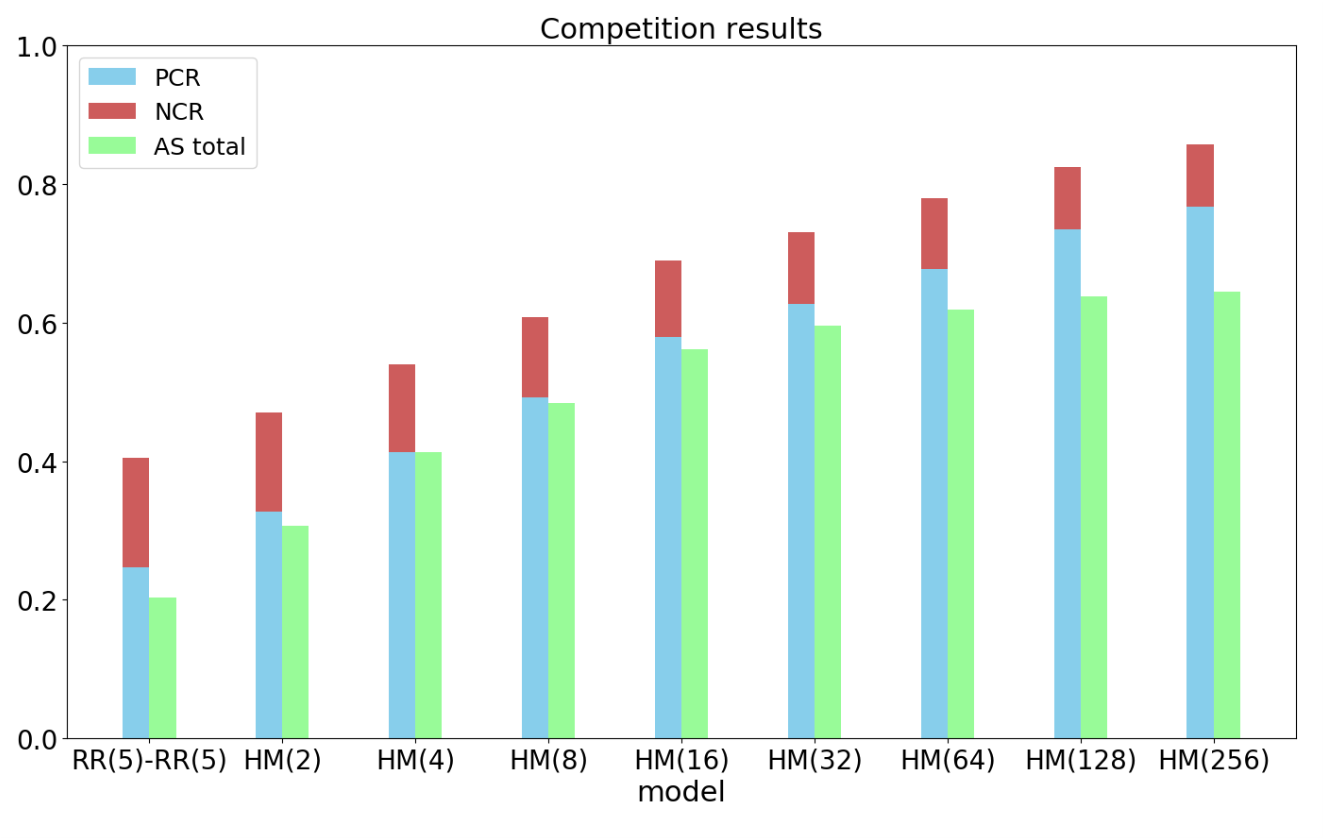
\includegraphics[width=\hsize]{chap3_HMs_total.png}
	\caption{Histogram for \textit{PCR, NCR, AS total} of Hierarchical Models(\textit{HM(n)})}
	\label{chap3_HMs_total}
\end{figure}
To clearly find out the difference between models, we use the indexes, \textit{PCR, NCR, AS total}. Fig.~\ref{chap3_HMs_total} shows the results to analyze \textit{HM(n)} with indexes. Blue color bar is for \text{PCR}, red color bar is for \text{NCR}, and green color bar is for \text{AS total}. Comparing \textit{HMs} with \textit{Basic model(RR(5)-RR(5))}, \textit{CR} \textit{PCR} and \textit{AS total} are all increased remarkably. \textit{HMs} have more positive consensus part than \textit{RR(5)-RR(5)}. But, \textit{HMs} have less negative consensus part than \textit{RR(5)-RR(5)}. It shows that as the number of B nodes are decreased, it is easy to make positive consensus(layer A opinion) and hard to make negative consensus(layer B opinion).  

In summary, all the Hierarchical Models have more consensus ratio than Random Regular Networks Model. However, positive consensus ratio is increased, but negative consensus ratio is decreased. It is found out that as the number of B nodes are more decreased, it makes easier to make positive consensus and harder to make negative consensus. In real world, it would be analyzed that as the number of leaders is less, social conflict are decreased and the opinion is convergent to social opinion(layer A). But, sometimes there are some dangers to ignore the leader opinion(layer B), or to cause more social conflict when there are stubborn leaders. 


\section{Competition on Networks with different number of internal links}
\begin{figure}[!htb]
	\centering
	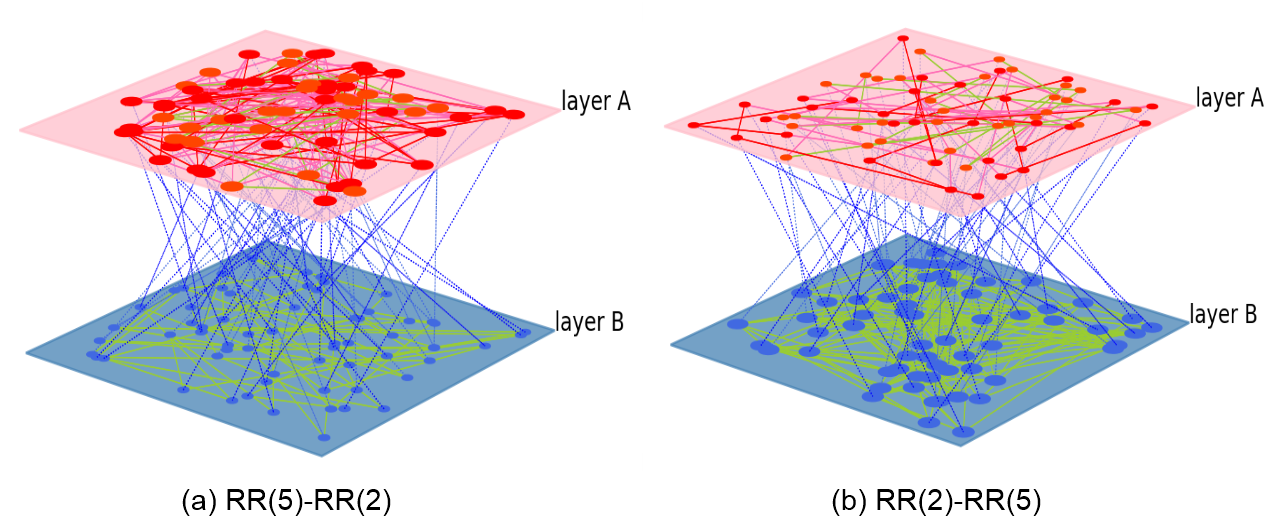
\includegraphics[width=\hsize]{chap3_changing_internal_edges.png}
	\caption{Competition on interconnected networks with different internal edges}
	\label{chap3_changing_internal_edges}
\end{figure}
Next, the interconnected networks are simulated with different internal degrees in order to define and evaluate the influence of internal degrees. Random regular network would be applied. And the number of internal degrees on each node is switched to various numbers as shown in Fig.~\ref{chap3_changing_internal_edges}. But, there is no change on external degree, which would be fixed to only $1$. Here, \textit{RR(n)-RR(m)} represents layer A has random regular network with $n$ internal edges, layer B has random regular network with $m$ internal edges.
\begin{figure}[!htb]
	\centering
	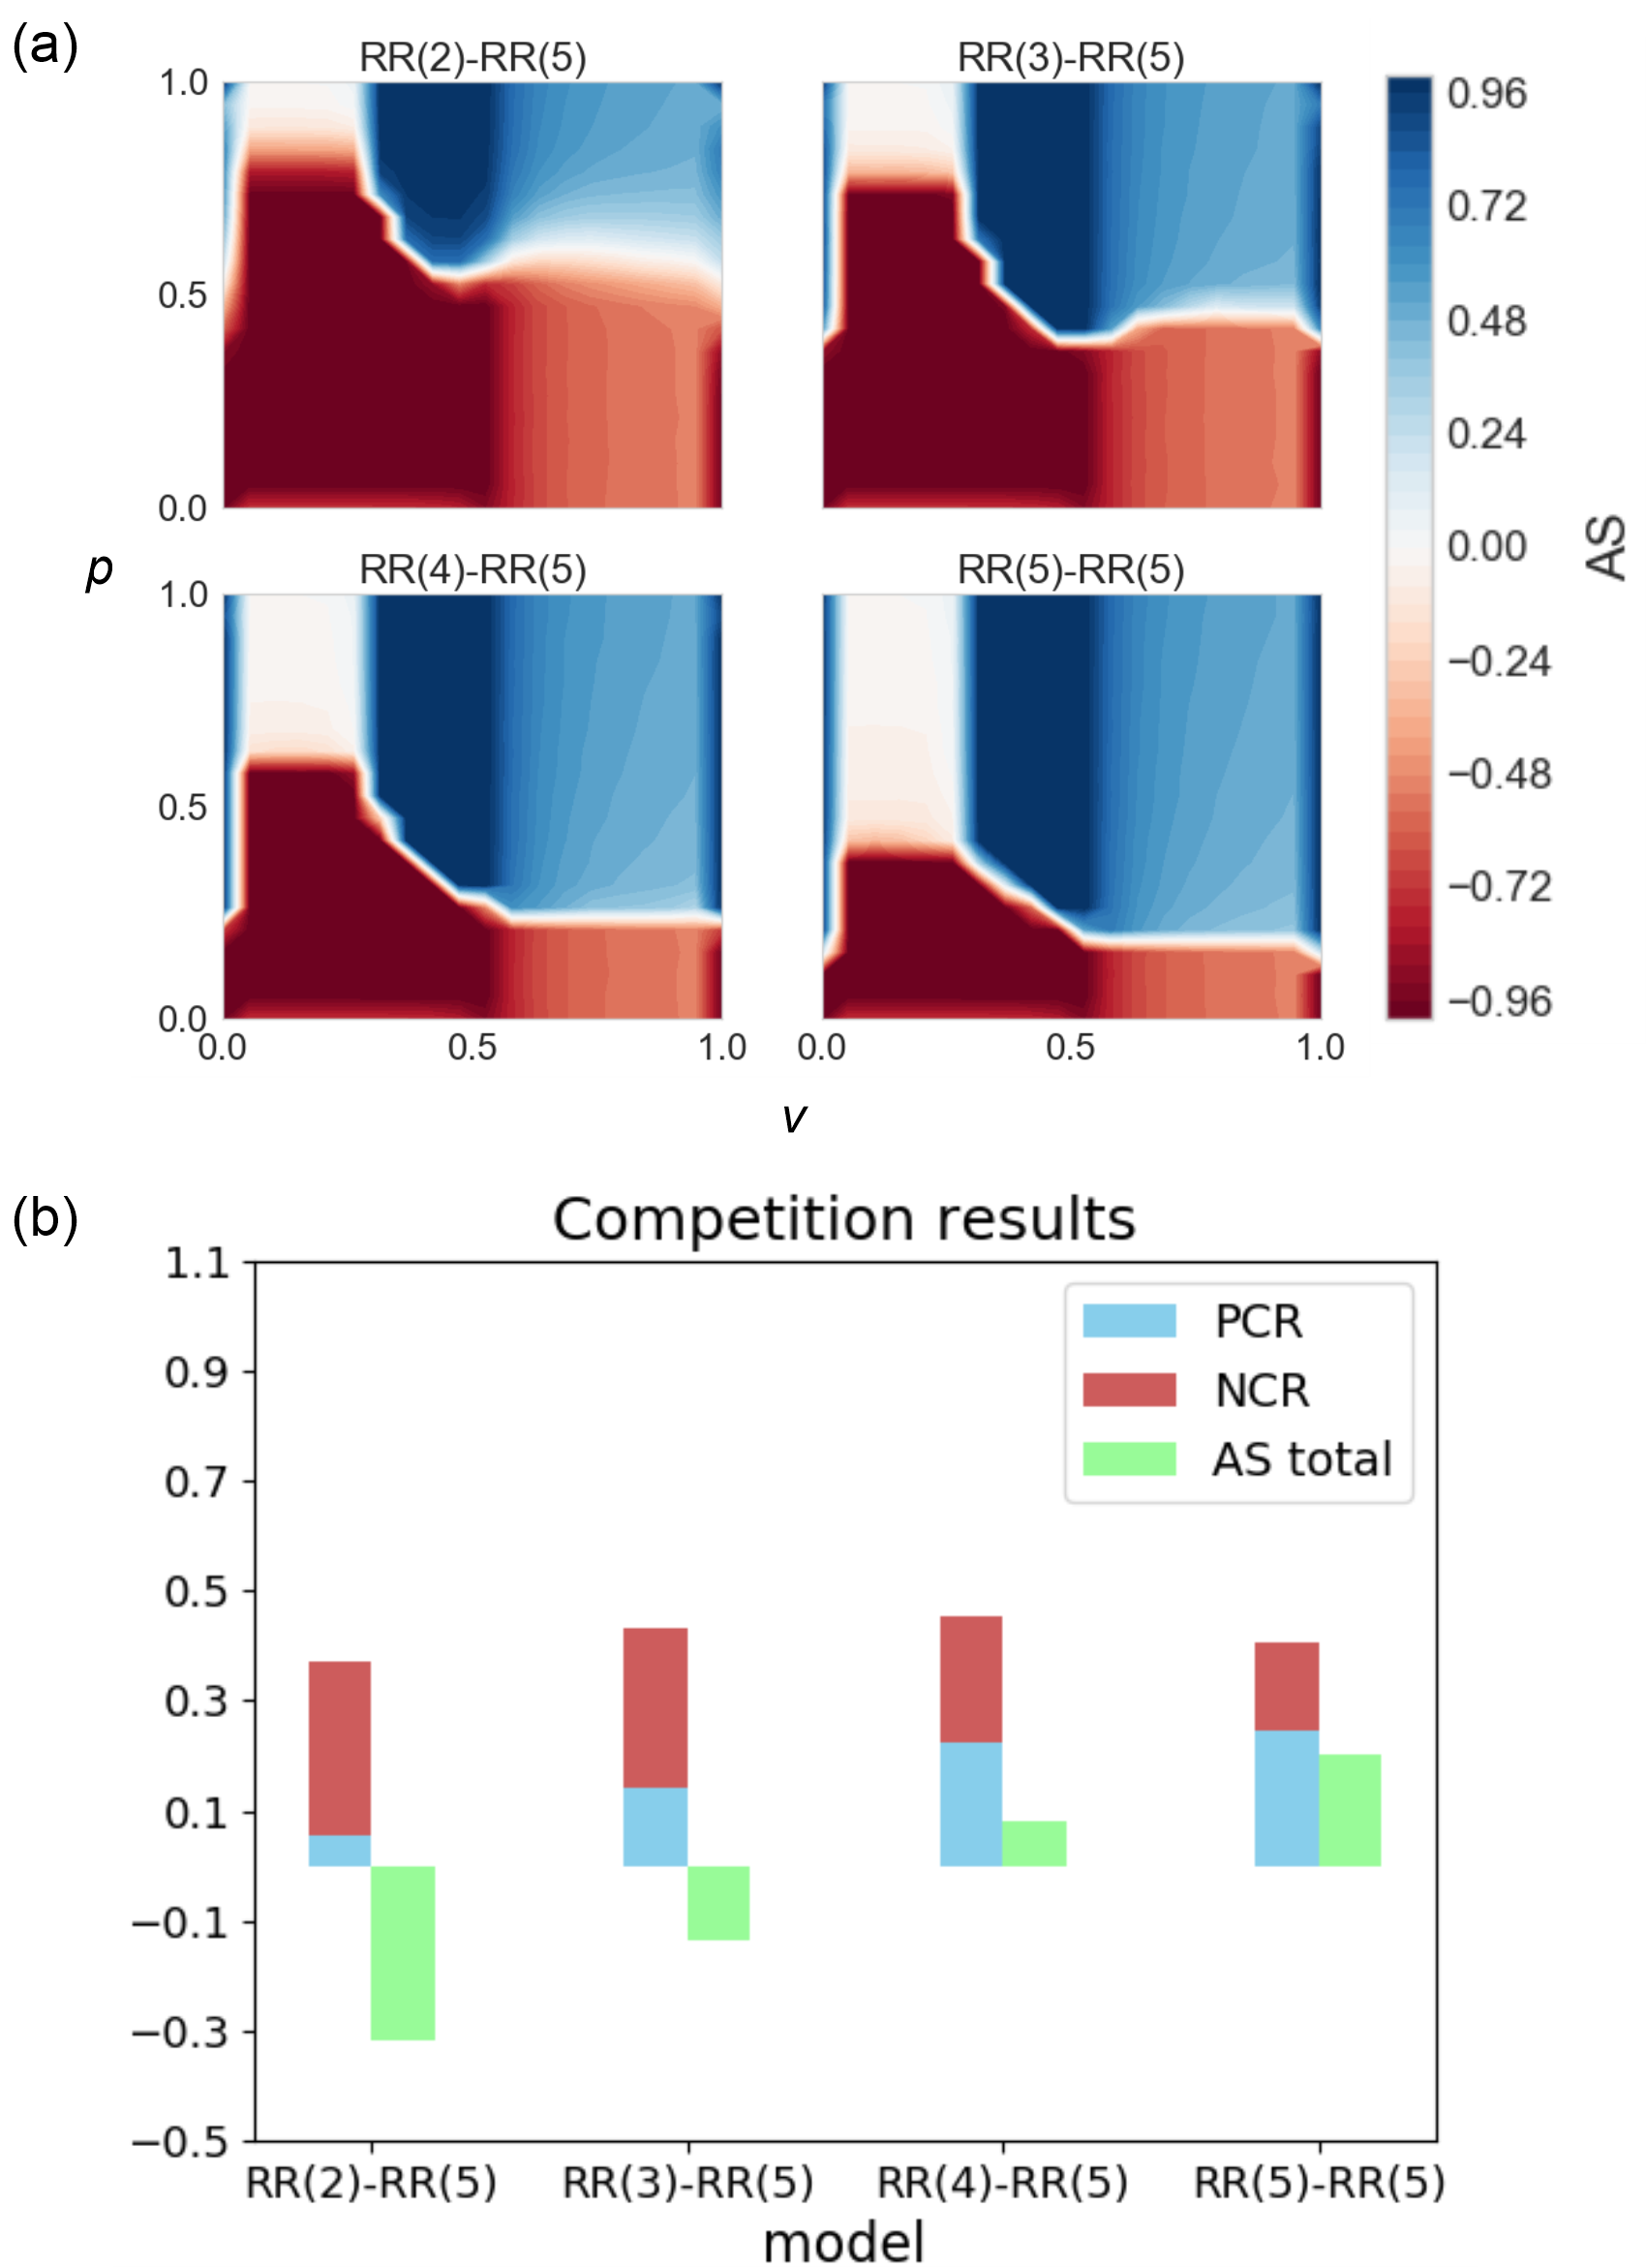
\includegraphics[width=\hsize]{chap3_internal_edge_A_total1.png}
	\caption{Simulation results with different internal degrees on layer A}
	\label{chap3_internal_edge_A_total}
\end{figure}
Firstly, the internal degrees on layer A are changed. The internal degrees on layer B are fixed to $5,120$, which means each node has $5$ internal degrees on layer B, and the internal degrees on layer A are switched into $2,048$, $3,072$, $4,096$, or $5,120$, which means each node has $2$, $3$, $4$, or $5$ internal degrees on layer A. Fig.~\ref{chap3_internal_edge_A_total} shows the simulation results for changing the internal degrees on layer A. As shows in Fig.~\ref{chap3_internal_edge_A_total} (a), as the number of internal degrees on layer A is increased, the red part is decreased and the blue part is increased.  

To clearly compare and analyze the results, the results are presented with the indexes, \textit{PCR, NCR, AS total} in Fig.~\ref{chap3_internal_edge_A_total} (b), which shows that as the number of internal degrees on layer A is increased, negative consensus is decreased and positive consensus is increased. As shown in Fig.~\ref{chap3_internal_edge_A_total}, RR(5)-RR(5) has the most \textit{PCR}, and RR(2)-RR(5) has the most \text{NCR}. However, \textit{CR} is almost same with all models in Fig.~\ref{chap3_interal_edge_A_total}. It can be analyzed that the number of internal degrees on layer A has the tendency to keep positive state and to change negative state into positive state. 
\begin{figure}[!htb]
	\centering
	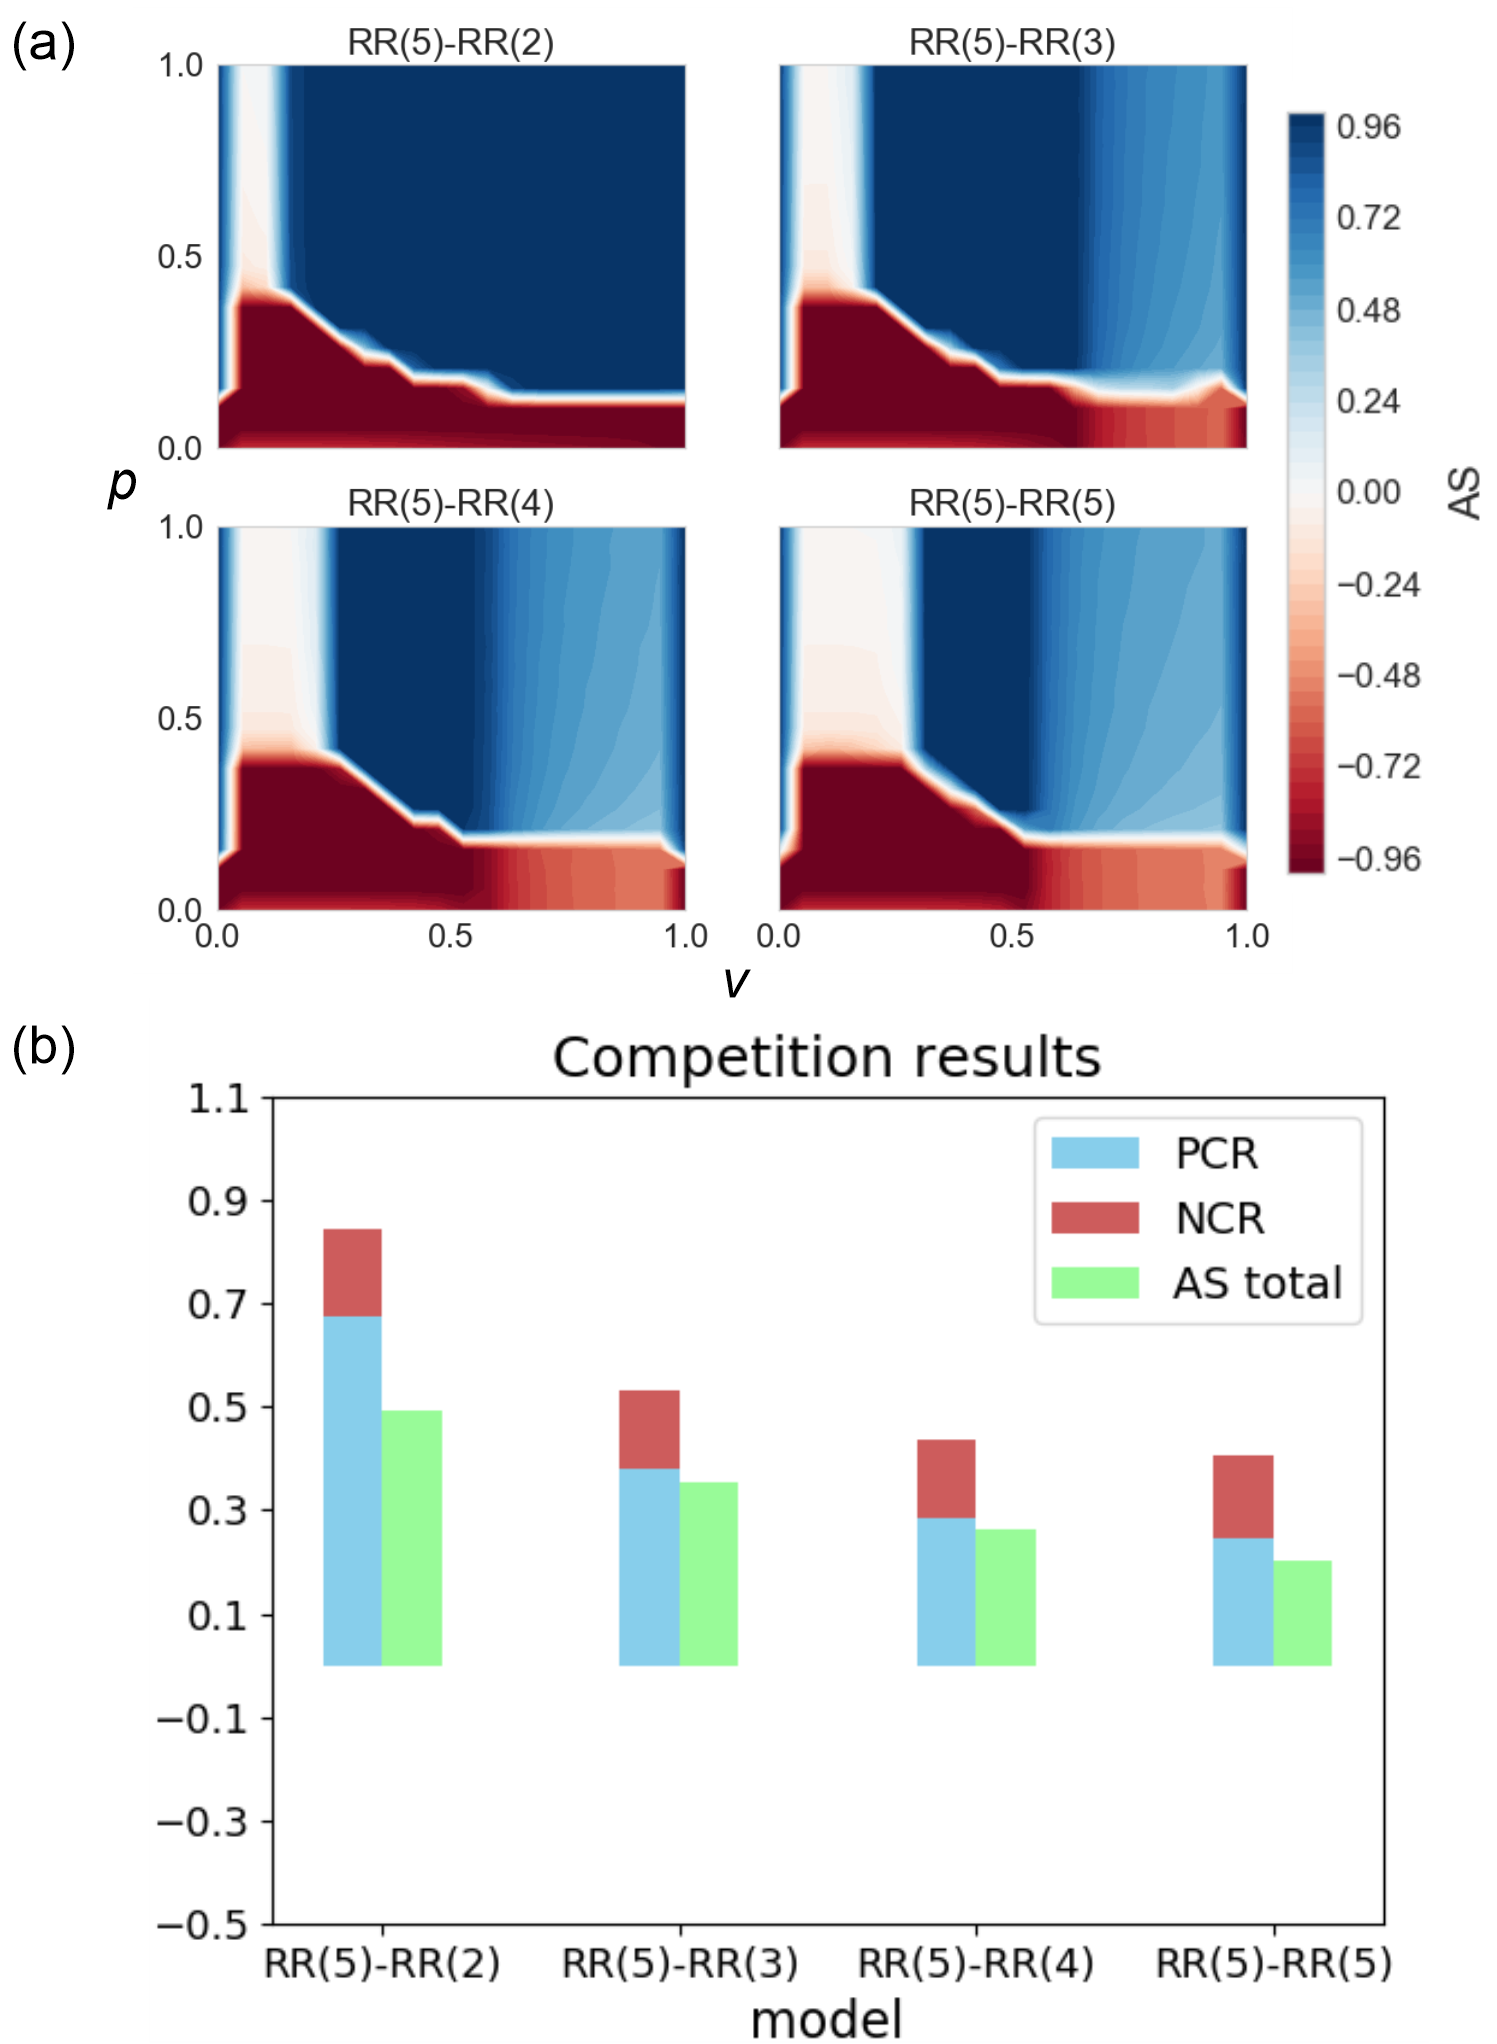
\includegraphics[width=\hsize]{chap3_internal_edge_B_total1.png}
	\caption{Simulation results with different internal degrees on layer B}
	\label{chap3_internal_edge_B_total}
\end{figure}
Next, the internal degrees on layer B are changed. The internal degrees on layer A are fixed to  $5,120$, which means each node has $5$ internal degrees on layer A, and the internal degrees on layer B are switched into $2,048$, $3,072$, $4,096$, or $5,120$, which means each node has $2$, $3$, $4$, or $5$ internal degrees on layer B.  
Fig.~\ref{chap3_internal_edge_B_total} shows the simulation results with changing the number of internal degrees on layer B. As shows in Fig.~\ref{chap3_internal_edge_B} (a), as the number of internal degrees on layer B is increased, the blue part is decreased, the white and light color part is increased, and the red part is almost same, though the shape of red area is changed.  As shown in Fig.~\ref{chap3_internal_edge_B_total} (b), RR(5)-RR(2) has the most \textit{PCR} and \textit{CR}, and RR(5)-RR(5) has the least \text{PCR} and \textit{CR}. However, \textit{NCR} is almost same with all models in Fig.~\ref{chap3_interal_edge_B_total}. It can be analyzed that the number of internal degrees on layer B has the tendency to hinder positive state and has the inverse relation with \textit{CR}. As the number of internal degrees on layer B is increased, \textit{PCR} and \textit{CR} is inversely decreased. It is recognized that the role of internal degrees on layer A is different with internal degrees on layer B. The internal degrees on layer A has the function to keep the state of layer A, and the internal degrees on layer B has the function to restrain the state of layer A and make coexistence part. 
\begin{figure}[!htb]
	\centering
	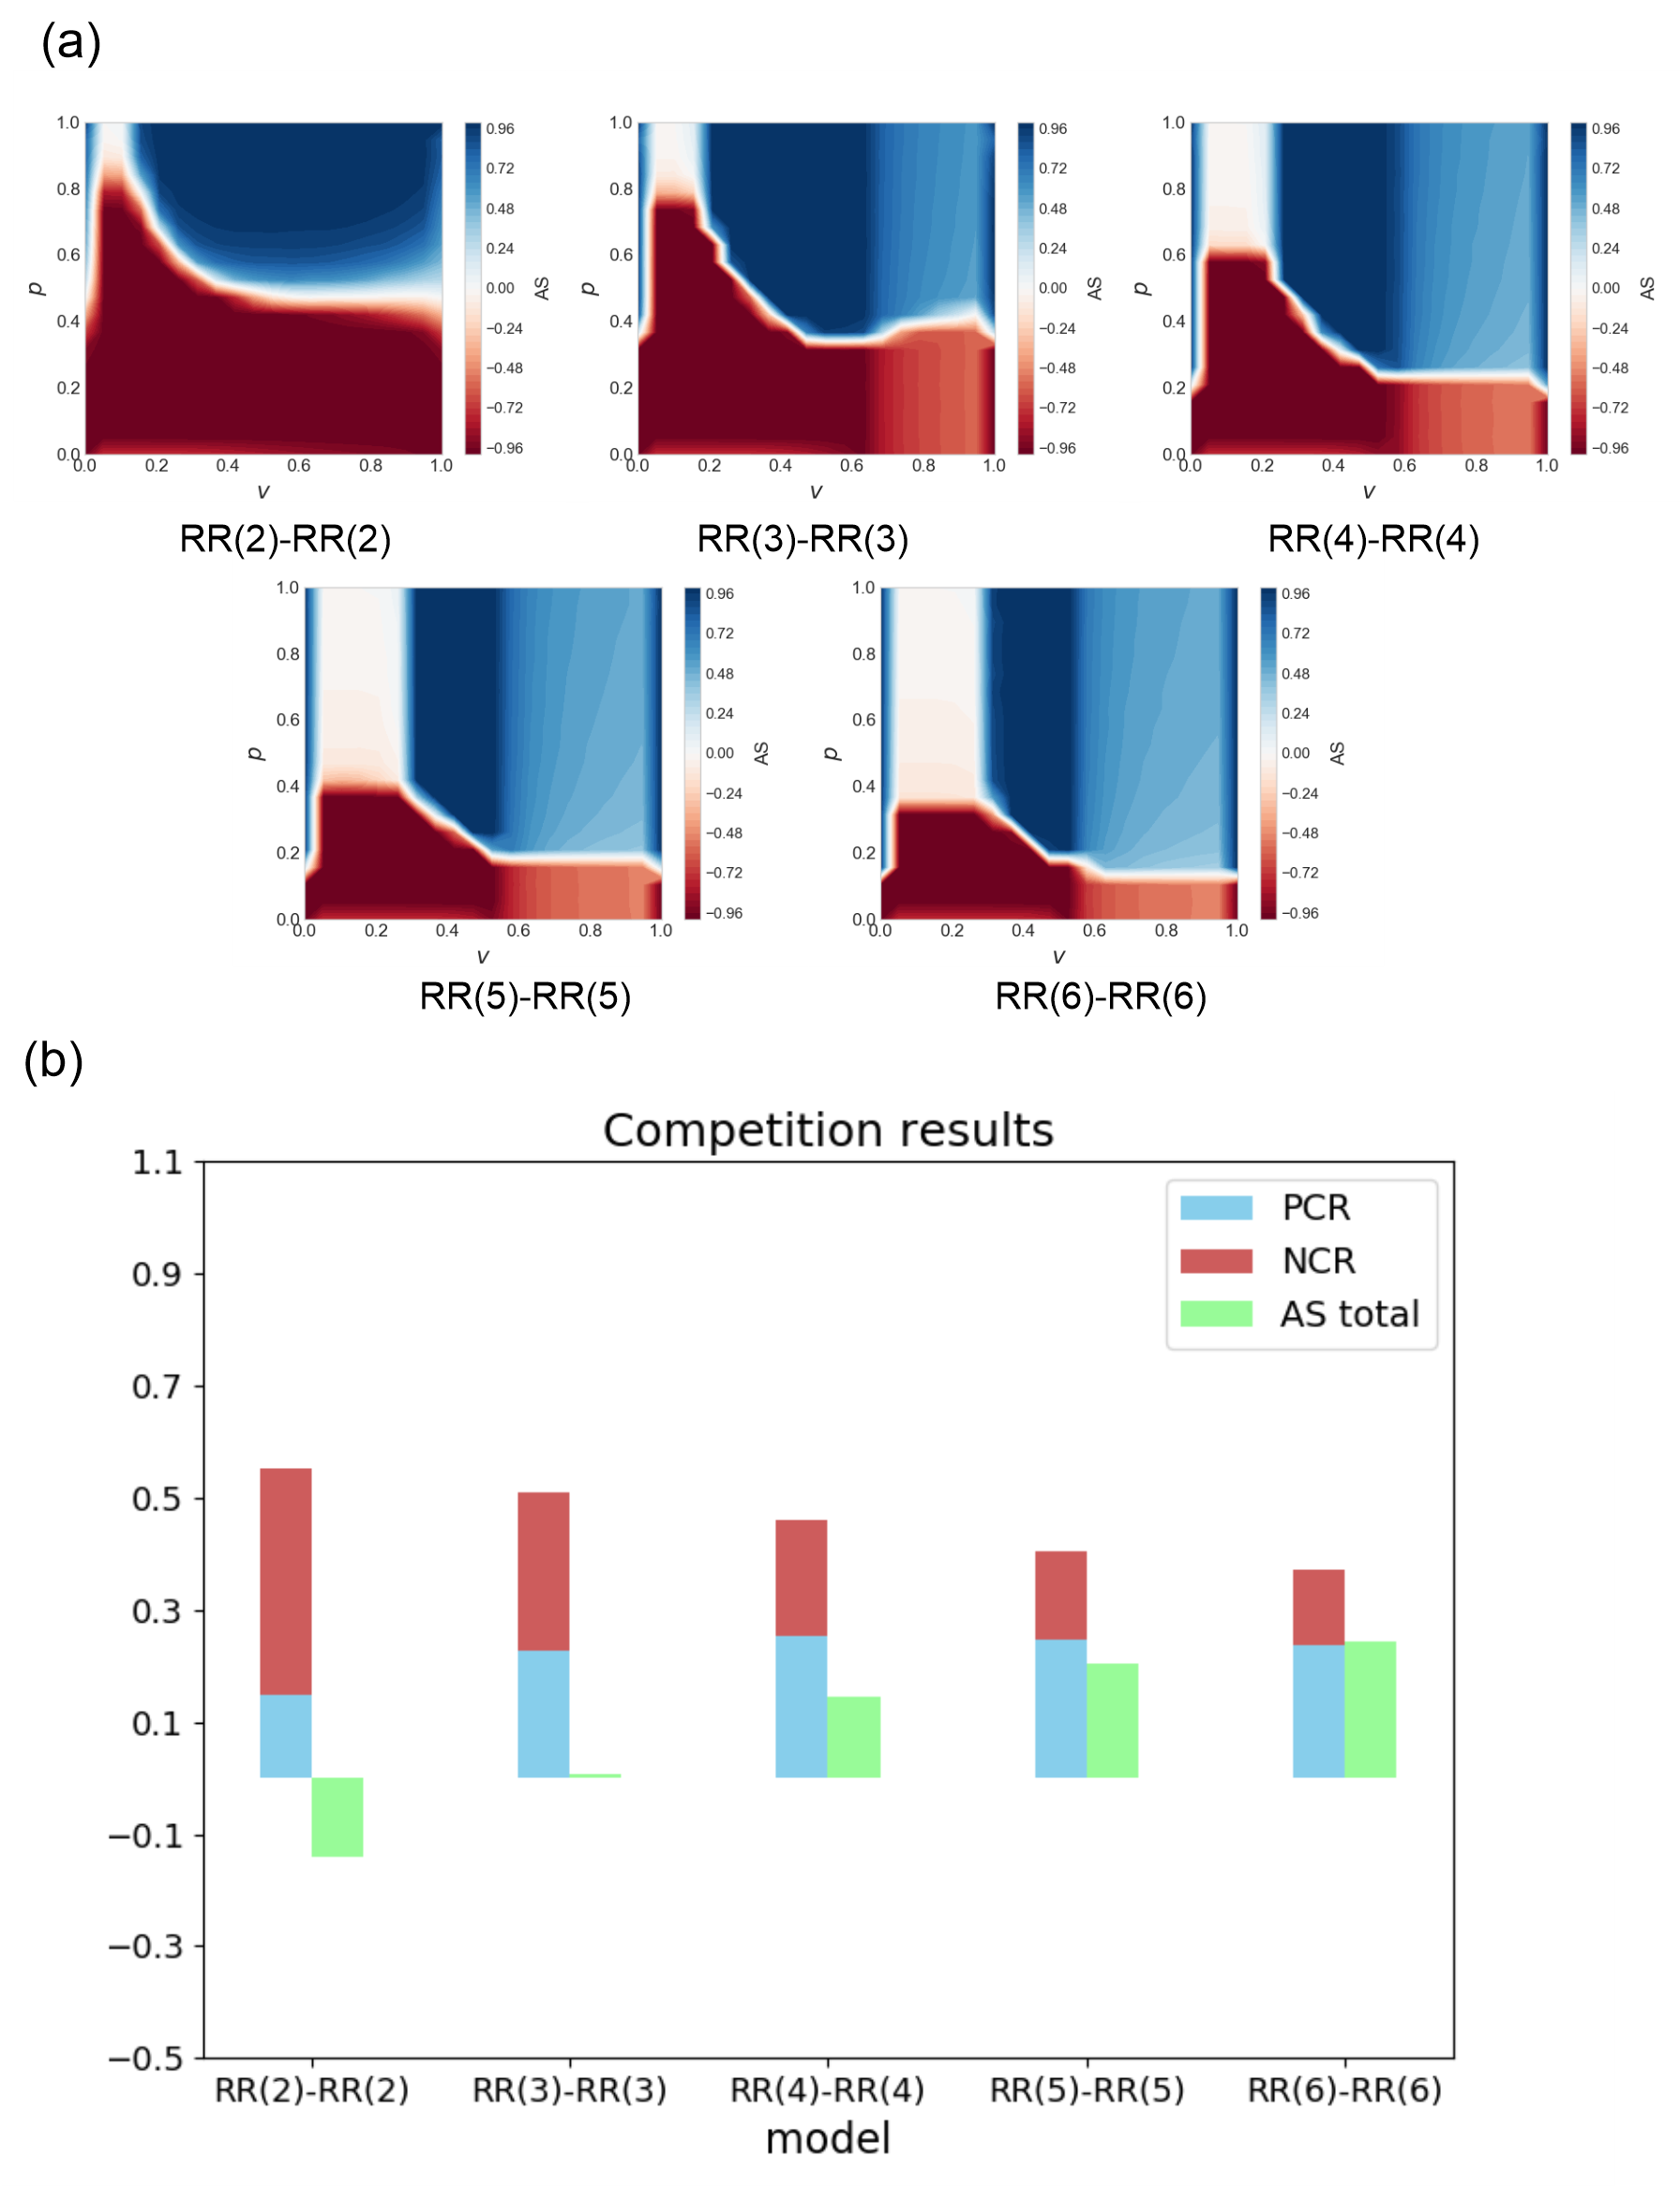
\includegraphics[width=\hsize]{chap3_internal_edge_two_total.png}
	\caption{Simulation results with changing internal degrees on both layers}
	\label{chap3_internal_edge_two_total}
\end{figure}
Next, it is simulated that internal degrees are changed on both layer A and layer B, such as RR(2)-RR(2), RR(3)-RR(3), RR(4)-RR(4), RR(5)-RR(5) and RR(6)-RR(6). Through these simulations, it would be found out that how total internal degrees affect the interconnected network.
Fig.~\ref{chap3_internal_edge_two_total} shows the influence of internal degrees on both layers. As the total number of internal degrees is increased, \textit{CR} is inversely decreased, and the ratio of positive consensus(blue area) is increased, but the ratio of negative consensus(red area) is decreased. It can be analyzed that a decrease in \textit{CR} is caused by increase in internal degrees on layer B, and an increase in ratio of \textit{PCR} is brought out by an increase in internal degrees on layer A. But, when the total number of internal degrees is increased, \textit{PCR, NCR, CR} indexes are decreased. It can be analyzed that too many internal degrees on both layers make it hard to reach consensus. 
\begin{figure}[!htb]
	\centering
	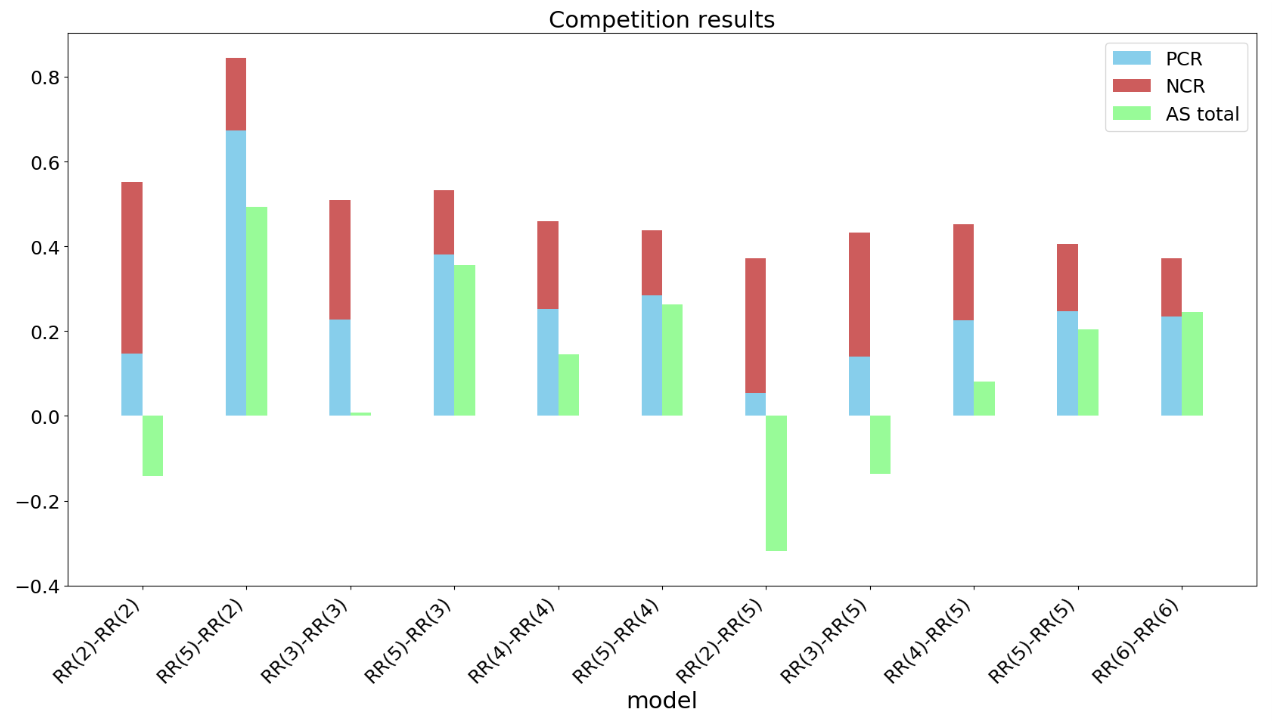
\includegraphics[width=\hsize]{chap3_internal_edge_AB_total.png}
	\caption{Total results with different internal degrees on two layers}
	\label{chap3_internal_edge_AB_total}
\end{figure}
In summary, 3 main simulations are implemented to find out the influence of internal degrees on interconnected network. First, the number of internal degrees on layer A are changed, and it is found out that the number of internal degrees on layer A has the tendency to keep positive state and to change negative state into positive state. Second, the number of internal degrees on layer B are switched, and it is found out that the number of internal degrees on layer B has the tendency to hinder positive state and has the inverse relation with \textit{CR}. Third, the number of internal degrees on both layers are changed, and it is found out that too many internal degrees make it hard to reach consensus. Fig.~\ref{chap3_internal_edge_AB_total} shows the result for all simulations. 
\begin{figure}[!htb]
	\centering
	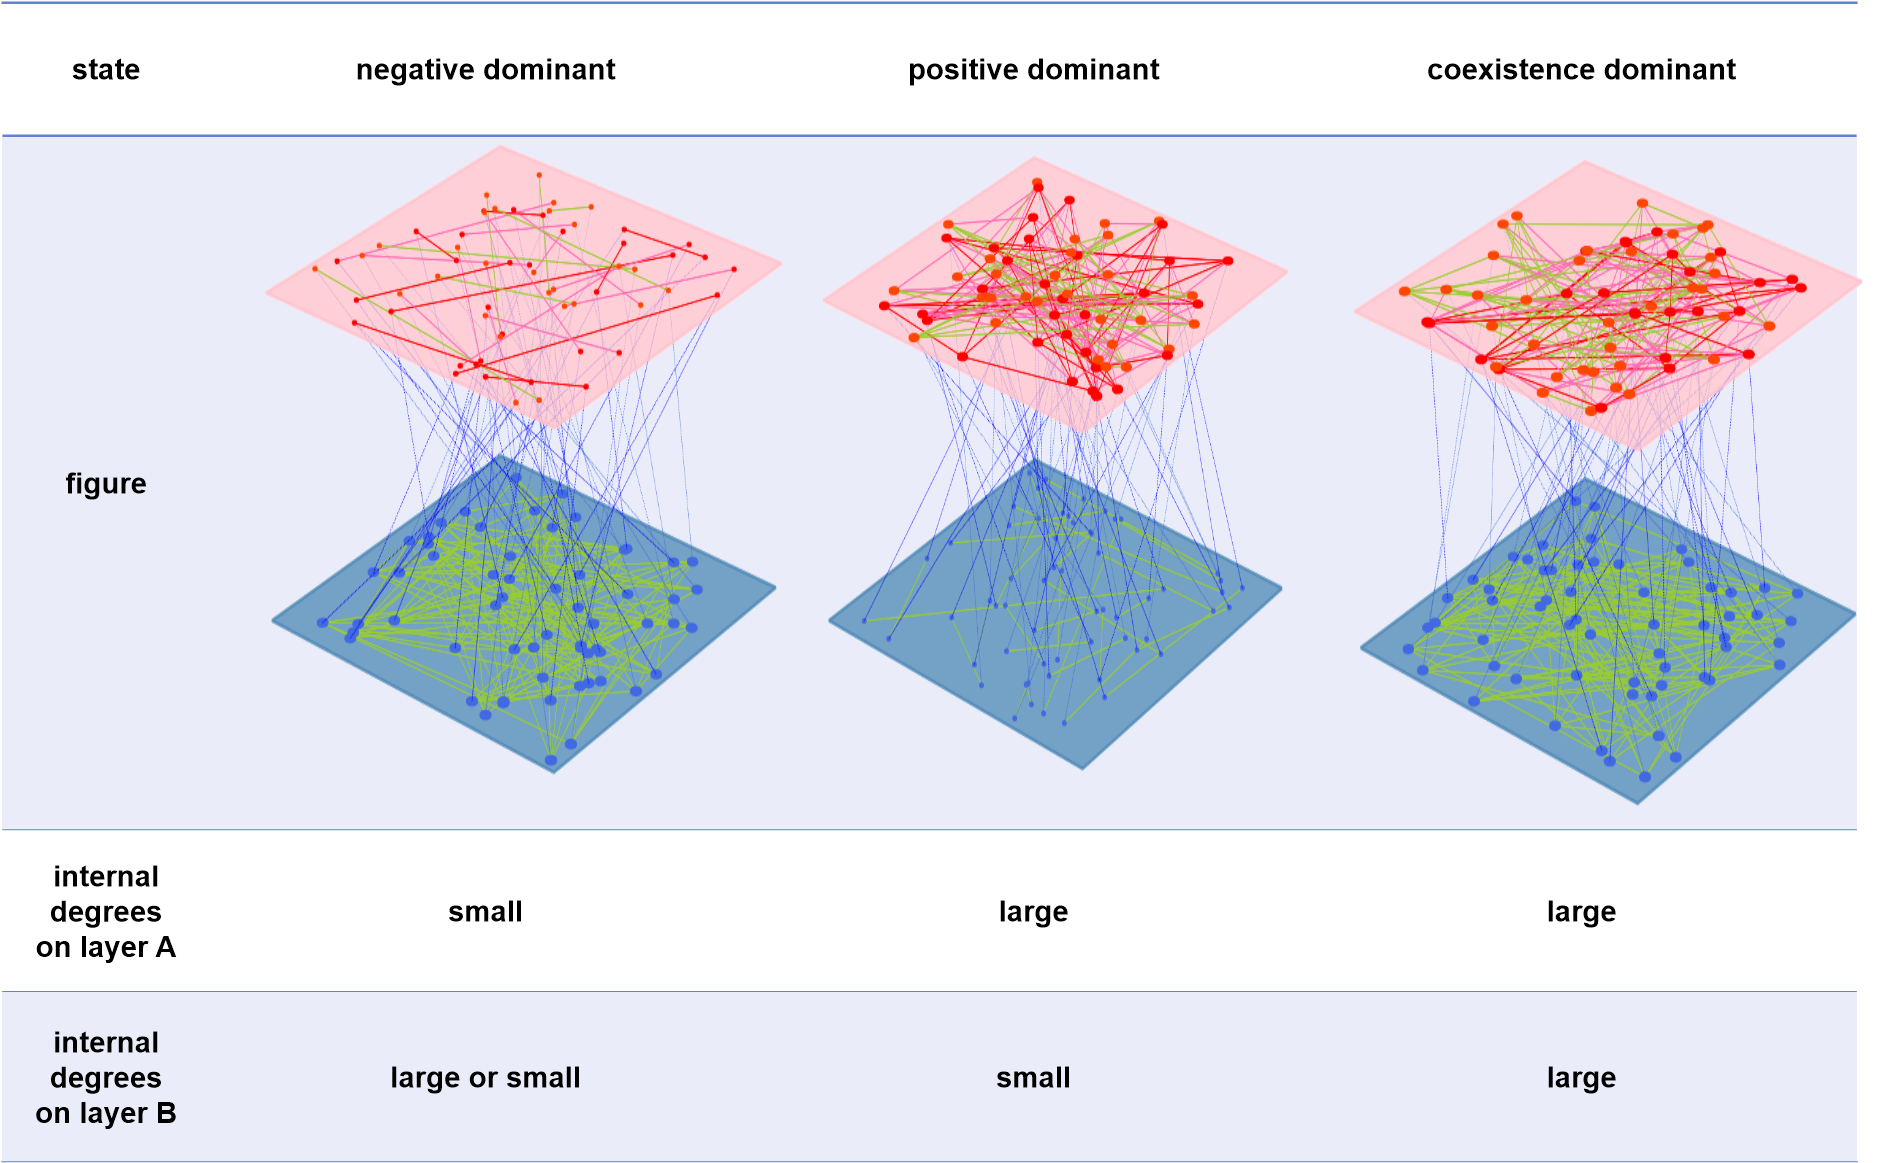
\includegraphics[width=\hsize]{chap3_internal_edge_summary.png}
	\caption{Categorizing network state according to internal degrees on two layers}
	\label{chap3_internal_edge_summary}
\end{figure}
Through these simulation results, we can analyze that how network state is changed according to the number of internal degrees. So, several conclusions can be arranged as shown in Fig.~\ref{chap3_internal_edge_summary}.  First, it is easy to reach negative consensus when the internal degrees on layer A is relatively small, but the internal degrees on layer B doesn't matter. Second, it is easy to make positive consensus when the internal degrees on layer A is relatively large and the internal degrees on layer B is relatively small. Third, social conflict can be caused when the internal degrees on both layers are too large.  

\section{Competition on networks with different structures}
\begin{figure}[!htb]
	\centering
	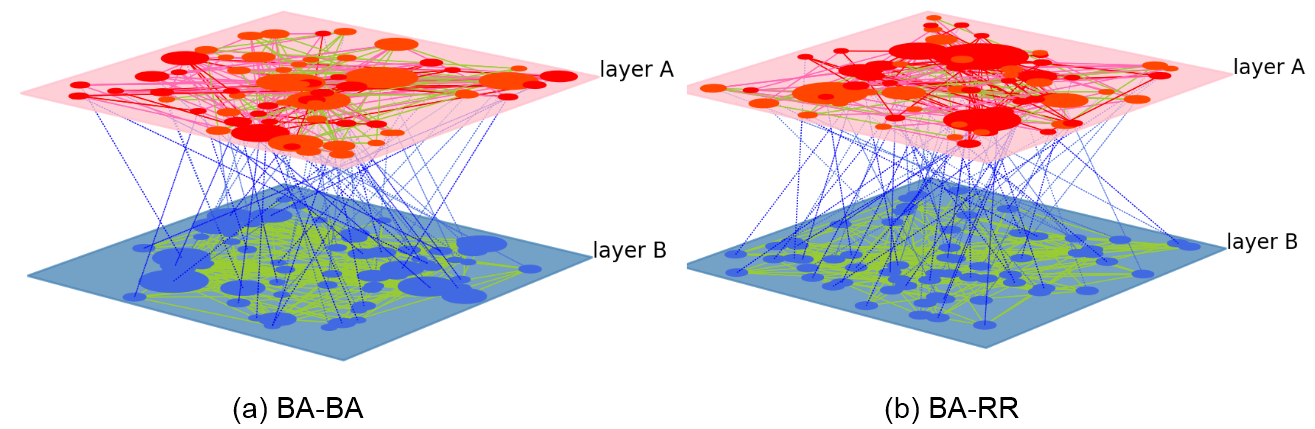
\includegraphics[width=\hsize]{chap3_changing_structure_type.png}
	\caption{Competition on interconnected networks with different structures}
	\label{chap3_changing_structure_type}
\end{figure}

So far, each layer of the interconnected network consisted of \textit{RR(random regular networks)} that has the same number of edges for each node. Now, the simulation would be implemented on different network type. Here, we use \textit{Barabasi-Albert network(BA)} structure as introduced in \parencite{barabasi1999}. \textit{Barabasi-Albert(BA)} network has $N$ nodes with attaching new nodes each with $K$ edges that are preferentially attached to existing nodes with high degrees. But, there is no change on external degree, which would be fixed to only $1$.
\begin{figure}[!htb]
	\centering
	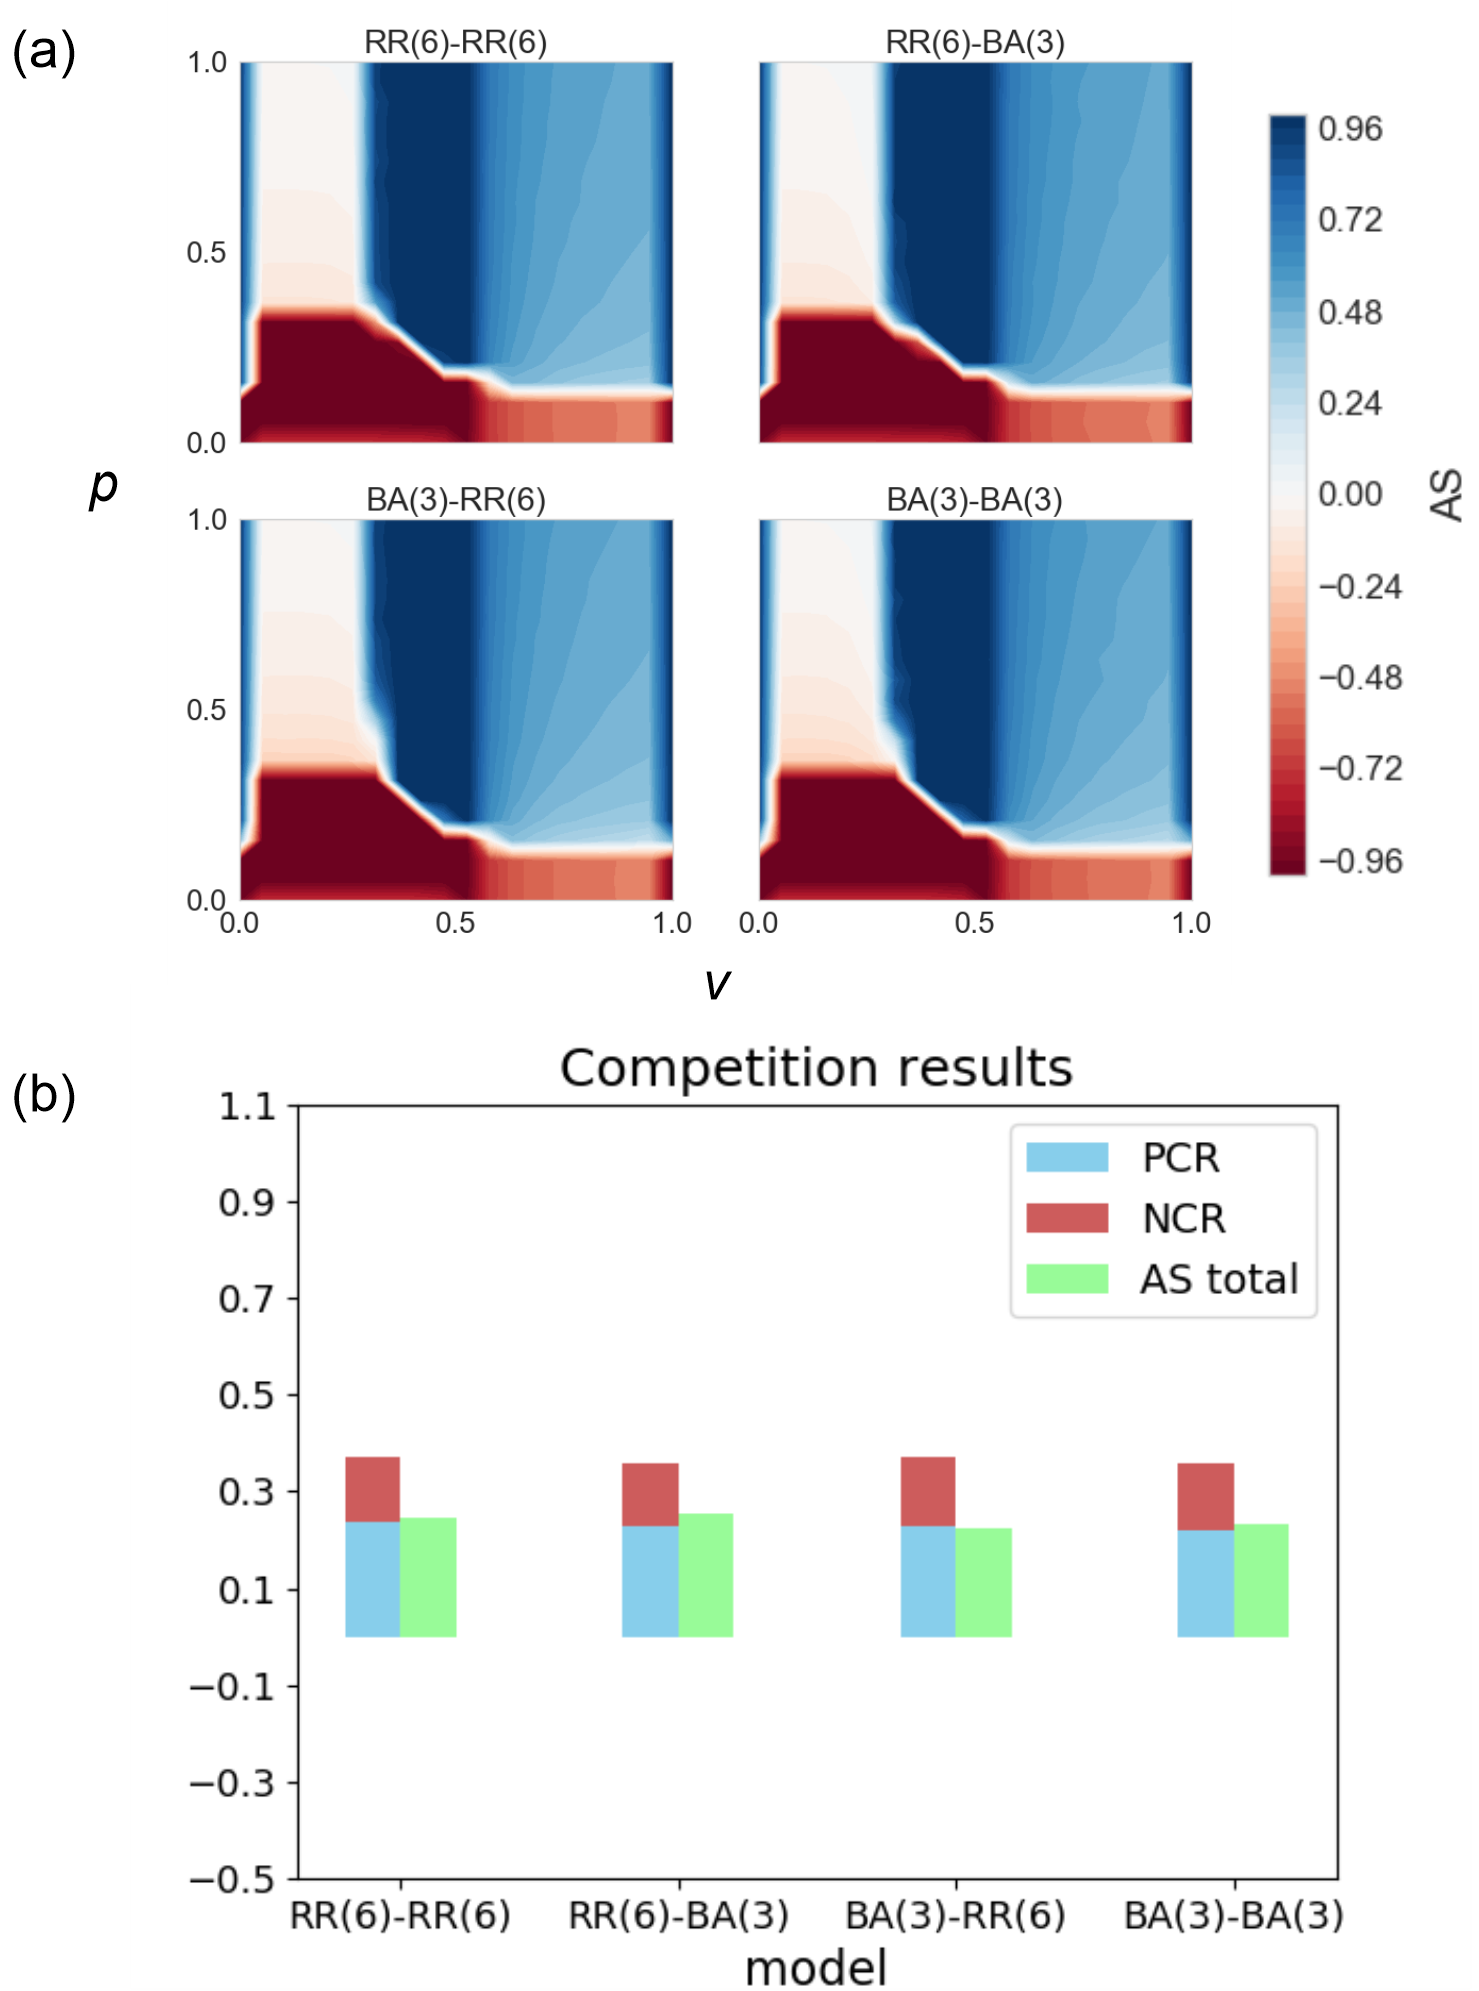
\includegraphics[width=\hsize]{chap3_changing_network_type11.png}
	\caption{Simulation results with different network types}
	\label{chap3_changing_network_type1}
\end{figure}

To evaluate the influence of network structure, 4 simulations are implemented with switching network structures. The \textit{BA} or \textit{RR} network is applied for both layers or switched on each layer. To restrain the influence of internal degree number, the number of internal degrees in \textit{BA} is set up to be similar with the number of internal degrees in \textit{RR}. The number of internal degrees in \textit{BA} is $6,135$, and the number of internal degrees in \textit{RR} is $6,144$. 
\begin{figure}[!htb]
	\centering
	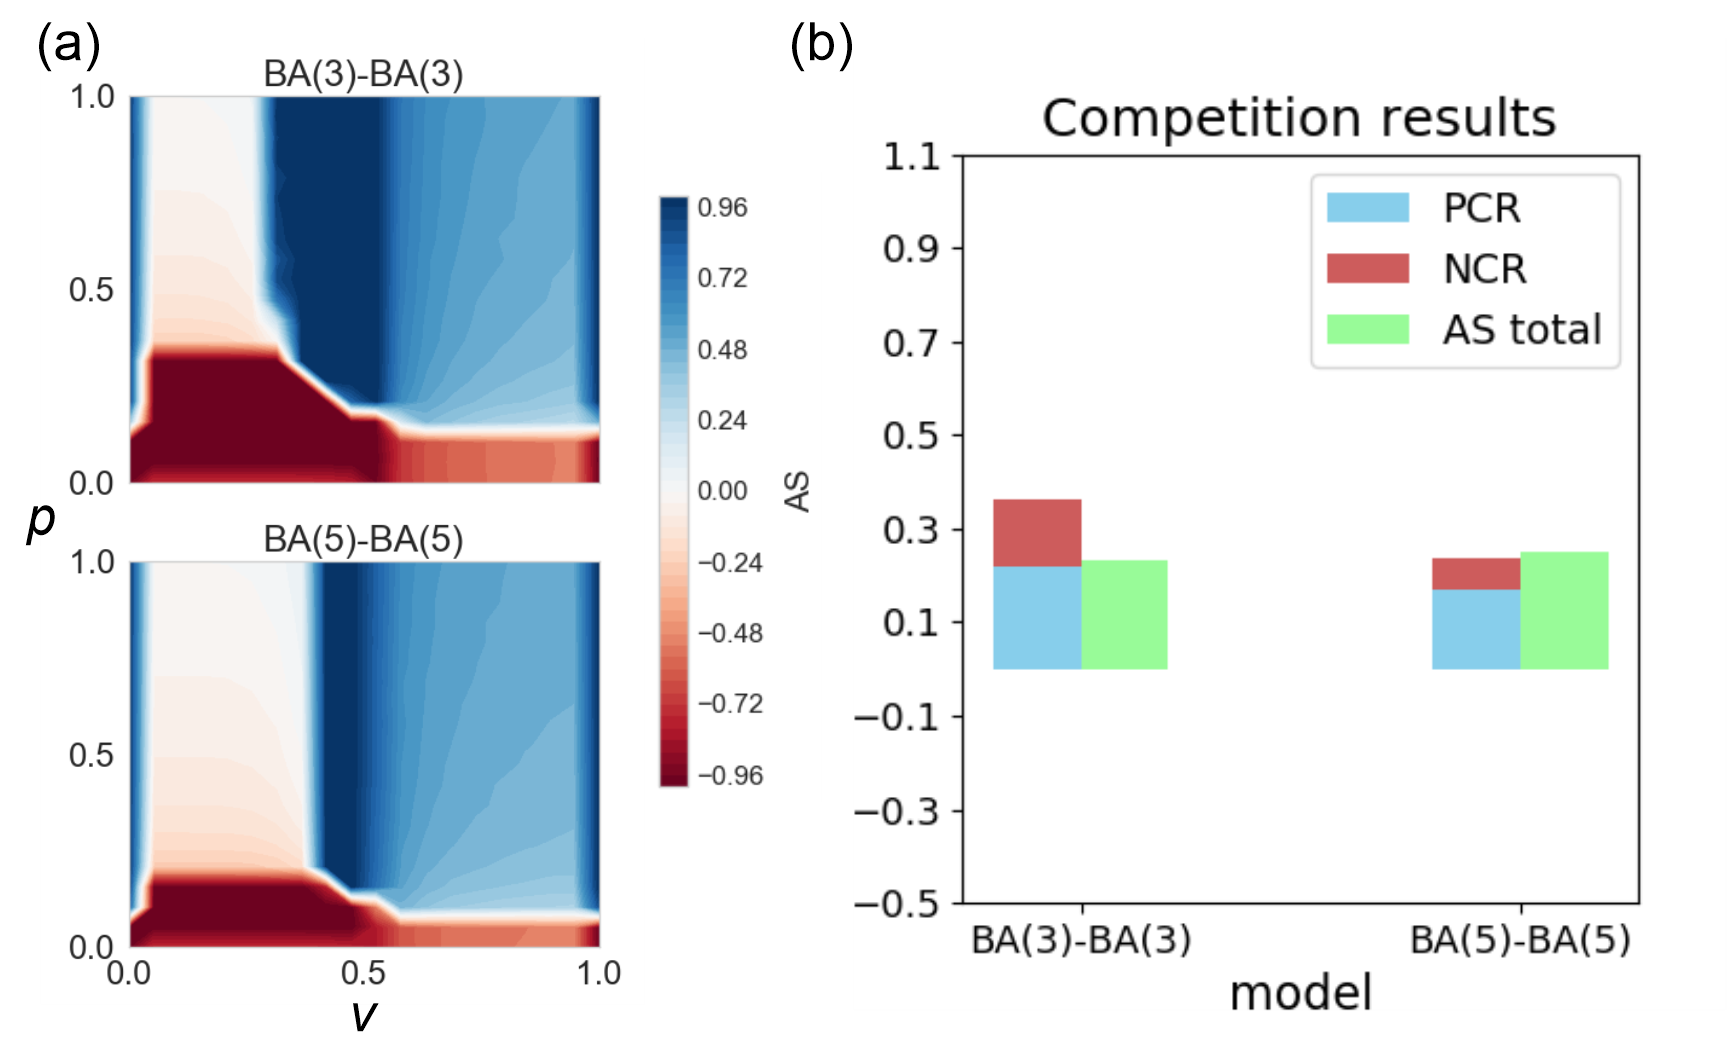
\includegraphics[width=\hsize]{chap3_changing_network_type2.png}
	\caption{BA-BA networks with changing internal degrees}
	\label{chap3_changing_network_type2}
\end{figure}
The simulation results are shown in Fig.~\ref{chap3_changing_network_type1}. The results of all simulations have almost the same features. The gap of \textit{PCR, NCR} and \textit{CR} is less than 0.02. The structure of network make no obvious difference of consensus results. Next, the number of internal degrees would be increased on the network, where consists of two \textit{BA}. It would be found out that how the number of internal degree work on different network type. 2 models, BA(3)-BA(3) and BA(5)-BA(5) would be simulated. BA(3)-BA(3) model has $6,135$ internal degrees on each layer, and BA(5)-BA(5) model has $10,215$ internal degrees on each layer. 


As shown in Fig.~\ref{chap3_changing_network_type2}, BA(5)-BA(5) has more coexistence area because of too many internal degrees. The influence of internal and external degrees number is more important to make network state and consensus than the influence of network type. However, If there are stubborn nodes on networks, the simulation results would be changed because node centrality of stubborn nodes would be changed according to network type. Finding key nodes on \textit{BA} network would be simulated and analyzed in chapter.~\ref{chap:finding key nodes on two layer networks}.

\section{Conclusion}
Various simulations have been simulated to find out the role of internal and external degrees and the influence of network types. All results of simulations are shown in Table.~\ref{Consensus properties of Simulation Models}. 
\begin{table}[!htb]
	\scriptsize
	\centering
    \caption{Consensus properties of Simulation Models}
	\label{Consensus properties of Simulation Models}
	\begin{center}
		\begin{tabular}{c|c|c|c|c|c|c|c|c} \hline\hline
			Div                    & A nodes& B nodes & A edges & B edges & AS total  & PCR    & NCR    & CR       \\ \hline \hline
			RR(2)-RR(5)            & 2,048  & 2,048   & 2,048   & 5,120   & -0.3186   & 0.0550 & 0.3175 & 0.3725   \\ \hline
			RR(3)-RR(5)            & 2,048  & 2,048   & 3,072   & 5,120   & -0.1368   & 0.1400 & 0.2925 & 0.4325   \\ \hline
			RR(4)-RR(5)            & 2,048  & 2,048   & 4,096   & 5,120   &  0.0804   & 0.2250 & 0.2275 & 0.4525   \\ \hline
			RR(5)-RR(2)            & 2,048 	& 2,048   & 5,120   & 2,048   &  0.4927   & 0.6725 & 0.1725 & 0.8450   \\ \hline	
			RR(5)-RR(3)            & 2,048 	& 2,048   & 5,120   & 3,072   &  0.3555   & 0.3800 & 0.1525 & 0.5325   \\ \hline
			RR(5)-RR(4)            & 2,048  & 2,048   & 5,120   & 4,096   &  0.2633   & 0.2850 & 0.1525 & 0.4375   \\ \hline
			RR(2)-RR(2)            & 2,048  & 2,048   & 2,048   & 2,048   & -0.1412   & 0.1475 & 0.4050 & 0.5525   \\ \hline
			RR(3)-RR(3)            & 2,048  & 2,048   & 3,072   & 3,072   &  0.0084   & 0.2275 & 0.2825 & 0.5100   \\ \hline
			RR(4)-RR(4)            & 2,048  & 2,048   & 4,096   & 4,096   &  0.1448   & 0.2525 & 0.2075 & 0.4600   \\ \hline
			RR(5)-RR(5)            & 2,048  & 2,048   & 5,120   & 5,120   &  0.2034   & 0.2475 & 0.1575 & 0.4050   \\ \hline
			RR(6)-RR(6)            & 2,048  & 2,048   & 6,144   & 6,144   &  0.2444   & 0.2350 & 0.1375 & 0.3725   \\ \hline
			RR(6)-BA(3)            & 2,048 	& 2,048   & 6,144   & 6,135   &  0.2541   & 0.2275 & 0.1300 & 0.3575   \\ \hline 
			BA(3)-RR(6)            & 2,048 	& 2,048   & 6,135   & 6,144   &  0.2242   & 0.2300 & 0.1425 & 0.3725   \\ \hline
			BA(3)-BA(3)            & 2,048 	& 2,048   & 6,135   & 6,135   &  0.2329   & 0.2200 & 0.1400 & 0.3600   \\ \hline
			BA(5)-BA(5)            & 2,048 	& 2,048   & 10,215  & 10,215  &  0.2496   & 0.1675 & 0.0675 & 0.2350   \\ \hline
			HM(2)  				   & 2,048 	& 1,024   & 5,120   & 2,560   &  0.3073   & 0.3275 & 0.1425 & 0.4700   \\ \hline    
			HM(4) 				   & 2,048 	&  512    & 5,120   & 1,280   &  0.4128   & 0.4125 & 0.1275 & 0.5400   \\ \hline
			HM(8)  				   & 2,048 	&  256    & 5,120   & 640     &  0.4846   & 0.4925 & 0.1150 & 0.6075   \\ \hline
			HM(16)				   & 2,048 	&  128    & 5,120   & 320     &  0.5610   & 0.5800 & 0.1100 & 0.6900   \\ \hline
			HM(32) 				   & 2,048 	&   64    & 5,120   & 160     &  0.5959   & 0.6275 & 0.1025 & 0.7300   \\ \hline
			HM(64) 				   & 2,048 	&   32    & 5,120   & 80      &  0.6185   & 0.6775 & 0.1025 & 0.7800   \\ \hline 
			HM(128) 			   & 2,048 	&   16    & 5,120   & 40      &  0.6379   & 0.7350 & 0.0900 & 0.8250   \\ \hline 
			HM(256) 			   & 2,048 	&    8    & 5,120   & 20      &  0.6454   & 0.7675 & 0.0900 & 0.8575   \\ \hline 
			 \hline
		\end{tabular}
	\end{center}
\end{table} 
Through the simulation results, several facts would be arranged like the followings. If there are no stubborn nodes, network types do not make different result for network state and consensus. But, we can provide three conclusions about the roles of internal and external degrees. First, hierarchical models show that it is easy to make consensus on both layers when the number of external edges in decision making is more than opinion layer. Second, the number of internal degrees on layer A has the tendency to keep positive state and to change negative state into positive state. Third,  the number of internal degrees on layer B has the tendency to hinder positive state. Forth, too many internal edges on each layer can cause inner conflict, and that makes it hard to have consensus state. We could apply these facts to make network structures or organization in real world. 